\documentclass[]{beamer}
\usepackage[utf8]{inputenc}
\usepackage{hyperref}
\usepackage{listings}
\lstset{
    basicstyle=\fontsize{10}{12}\selectfont\ttfamily,
    keywordstyle=\color{blue},
    breaklines=true,
    showtabs=false,
    showstringspaces=false,
    numberstyle=\tiny\color{mygray}
}
\usepackage{pslatex}        % for better PDF on screen
%\usepackage{textcomp}

%\usetheme{AnnArbor}
%\usetheme{Antibes}
%\usetheme{Berkeley}
%\usetheme{Berlin}
%\usetheme{Boadilla}
\usetheme{CambridgeUS}
%\usetheme{Copenhagen}
%\usetheme{Dresden}
%\usetheme{Frankfurt}
%\usetheme{Goettingen}
%\usetheme{Hannover}
%\usetheme{JuanLesPins}
%\usetheme{Marburg}
%\usetheme{Montpellier}
%\usetheme{PaloAlto}
%\usetheme{Pittsburgh}
%\usetheme{Rochester}
%\usetheme{Singapore}
%\usetheme{Szeged}
%\usetheme{Warsaw}

% Force full screen
% \hypersetup{pdfpagemode=FullScreen}

% Navigation menu
\setbeamertemplate{navigation symbols}{%
%     \insertslidenavigationsymbol
%     \insertframenavigationsymbol
%     \insertsubsectionnavigationsymbol
%     \insertsectionnavigationsymbol
%     \insertdocnavigationsymbol
%     \insertbackfindforwardnavigationsymbol
}


% contenu de la page de titre
\title[Deconstructing some challenges from LCSC 2019]{Lëtz Cybersecurity Challenge 2019}
\subtitle{Deconstructing some challenges}
\author{C\'{e}dric Bonhomme}
\institute[CIRCL]{CIRCL - Security Made In Lëtzebuerg}
\date{March 09, 2019}

% \logo{
\includegraphics[height=0.5cm]{./images/logo.png}}
\newsavebox{\logoA}
\newsavebox{\logoB}
\savebox{\logoA}{
\includegraphics[width=2.5cm]{./images/logo-circl.png}}
\savebox{\logoB}{
\includegraphics[width=2.5cm]{./images/logo.png}}
\titlegraphic{%
  \raisebox{.5\dimexpr\ht\logoB-\ht\logoA}{\usebox{\logoA}}% raise smaller logo into position
  \hspace*{5cm}%
  \usebox{\logoB}
}
% End of preamble


\begin{document}
\begin{frame}
    \titlepage
\end{frame}


%
% SECTION: What is this workshop about?
%
\section*{What is this workshop about?}
\begin{frame}
    \frametitle{What is this workshop about?}
    \begin{center}
        \begin{itemize}
            \item we will present and deconstruct \href{https://github.com/cscluxembourg/vestatech}{some challenges} of the Lëtz Cybersecurity Challenge 2019;
            \item in the framework of the ENISA European Cyber Security Challenge;
            \item not yet registered ? Let's go: \href{https://vestatech.cybersecuritychallenge.lu}{https://vestatech.cybersecuritychallenge.lu}
        \end{itemize}
    \end{center}
\end{frame}


% --------- Summary ---------
\begin{frame}
    \frametitle{Contents}
    \begin{columns}[t]
        \begin{column}{5cm}
            \tableofcontents[sections={1-3}]
        \end{column}
        \begin{column}{5cm}
            \tableofcontents[sections={4-5}]
        \end{column}
    \end{columns}
\end{frame}
% ----------------------------



%
% SECTION: Network analysis
%
\section{Network analysis}
\begin{frame}
    \frametitle{Network analysis}
    \begin{columns}[t]
        \begin{column}{5cm}
            \tableofcontents[sections={1-3}, currentsection, hideothersubsections]
        \end{column}
        \begin{column}{5cm}
            \tableofcontents[sections={4-5}, currentsection, hideothersubsections]
        \end{column}
    \end{columns}
\end{frame}
 
\subsection{Related challenge}
\begin{frame}
\frametitle{Related challenge}
\begin{itemize}
    \item \href{https://github.com/cscluxembourg/vestatech/blob/master/challenges/find-the-author/gift.cap}{Find the author. The line was not secured.} - 1 star (super easy);
\end{itemize}
\bigskip
How did you solved this challenge?

\bigskip
From the feedbacks we got it seems that the majority of participants used Wireshark.
\end{frame}


\subsection{Presentation}
\begin{frame}
\frametitle{Presentation}
\framesubtitle{}
\begin{itemize}
\item tcpdump, BPF, Wireshark;
\item little exercices with BPF filters, etc. solution of the challenge.
\end{itemize}
\end{frame}




\begin{frame}
\frametitle{Wireshark}
\begin{itemize}
    \item Wireshark is a graphical network packet analysis tool.
    \item promiscious mode: ifconfig eth0 promisc
    \item other interception methods: bridge interception, honeypot, etc.
\end{itemize}
\end{frame}

\begin{frame}
\frametitle{Wireshark}
\framesubtitle{Follow TCP stream}
\begin{center}
    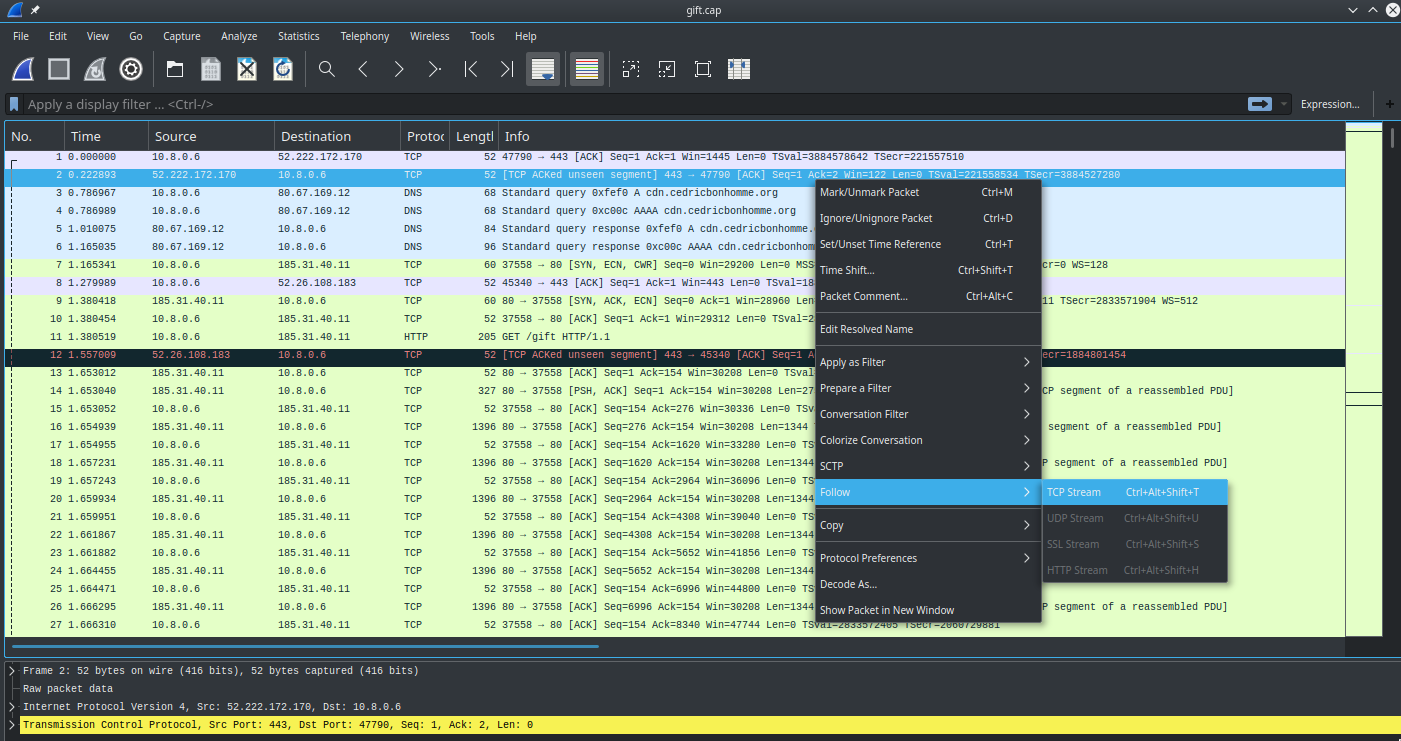
\includegraphics[height=6.5cm, width=12.0cm]{./images/Wireshark_follow_tcp_stream.png}
\end{center}
\end{frame}

\begin{frame}
\frametitle{Wireshark}
\framesubtitle{Search for specific packets}
\begin{itemize}
    \item \texttt{frame contains "gift"};
    \item \texttt{tcp.port == 443};
    \item \texttt{dns.resp.len > 0};
    \item \texttt{ip.addr == 52.7.23.87}.
\end{itemize}
\end{frame}

\begin{frame}
\frametitle{tcpdump and Berkeley Packet Filter}
\framesubtitle{}
\begin{itemize}
    \item BPF provides a raw interface to data link layers (between link-level driver and the user space);
    \item \texttt{tcpdump -i eth0 -vv 'tcp[0:2] > 1024'}: matching any TCP traffic with a source port $>$ 1024;
    \item 
\end{itemize}
\end{frame}


\begin{frame}
\frametitle{Solution with Wireshark}
\begin{center}
    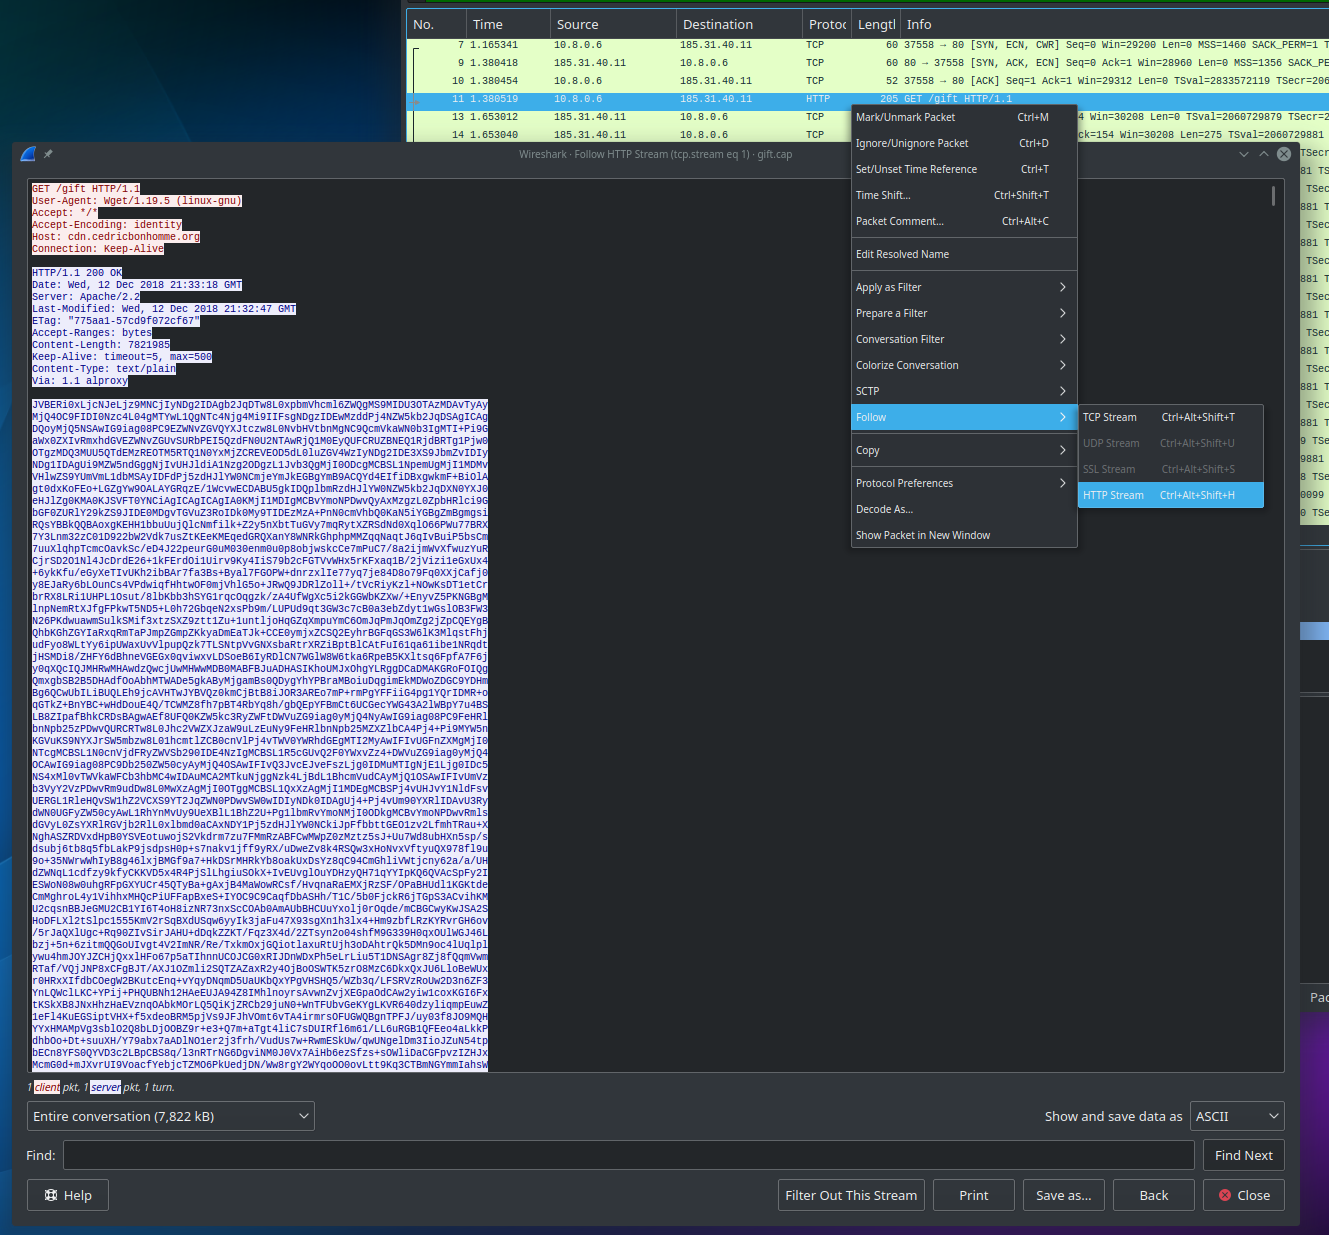
\includegraphics[height=6.5cm, width=12.0cm]{./images/Wireshark_follow_http_stream.png}
\end{center}
The size of the pcap is \textit{almost} the size of the data...
\end{frame}
 


\begin{frame}[fragile]
\frametitle{A pythonic solution}
\begin{lstlisting}[language=Python]
#! /usr/bin/python
# -*- coding: utf-8 -*-

# tcpflow -r gift.cap

with open("185.031.040.011.00080-010.008.000.006.37558" ,
            "r") as flow:
    data = flow.readlines()

for i, line in enumerate(data):
    if "Content-Type" in line:
        file_type = line.split("/")[1]
        with open("result", "w") as result:
            result.write("".join(data[i+1:]))
            exit()
\end{lstlisting}
\end{frame}
 


 

 
 

 
%
% SECTION: Gentle introduction to RSA
%
\section{Gentle introduction to RSA}
\begin{frame}
    \frametitle{Gentle introduction to RSA}
    \begin{columns}[t]
        \begin{column}{5cm}
            \tableofcontents[sections={1-3}, currentsection, hideothersubsections]
        \end{column}
        \begin{column}{5cm}
            \tableofcontents[sections={4-5}, currentsection, hideothersubsections]
        \end{column}
    \end{columns}
\end{frame}

\subsection{Related challenges}
\begin{frame}
\frametitle{Related challenges}
\begin{itemize}
    \item \href{https://github.com/cscluxembourg/vestatech/blob/master/challenges/Sergei_forgot_his_formula/wip.py}{Sergei forgot his formula} - 2 stars;
    \item \href{https://github.com/cscluxembourg/vestatech/tree/master/challenges/A_key_from_the_past}{A key from the past} - 3 stars.
\end{itemize}
\bigskip
How did you solved these challenges?
\end{frame}

\begin{frame}
\frametitle{Related challenges - Sergei forgot his formula}
\framesubtitle{Do you know how is generated a RSA key?}
\begin{center}
    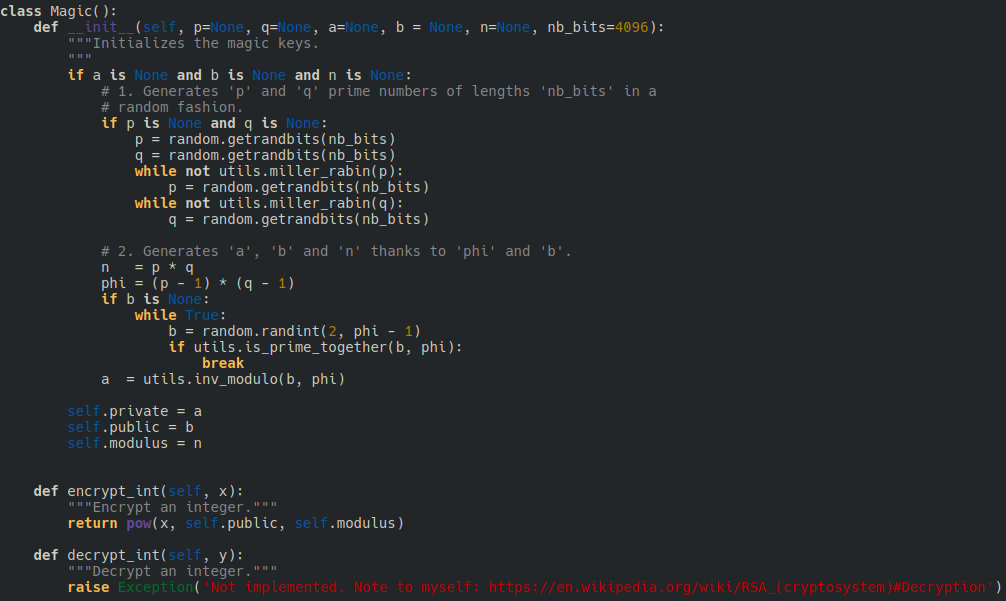
\includegraphics[height=6.2cm, width=12.0cm]{./images/RSA-algo-key-generation.png}
\end{center}
\href{https://en.wikipedia.org/wiki/RSA_(cryptosystem)\#Decryption}{Super easy} ;-)
\end{frame}


\begin{frame}
\frametitle{Related challenges - A key from the past}
\framesubtitle{A weakness of RSA: the \textit{quality} of your key}
\begin{center}
    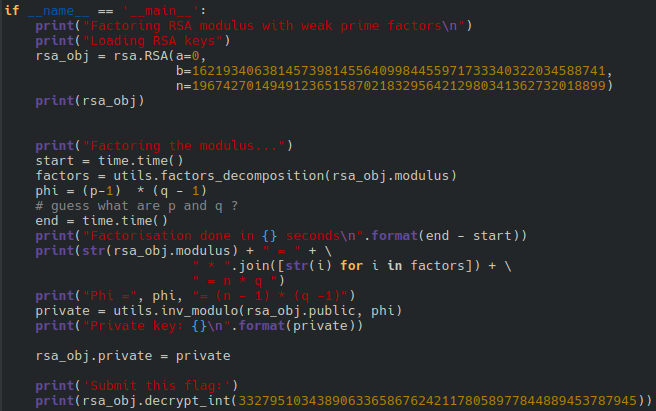
\includegraphics[height=6.2cm, width=12.0cm]{./images/RSA-weak-prime-factors.png}
\end{center}
And random implementation flaws...
\end{frame}



\subsection{Presentation}
\begin{frame}
\frametitle{Presentation}
\framesubtitle{Diffie}
\begin{columns}
    \begin{column}{5cm}
        \begin{center}
            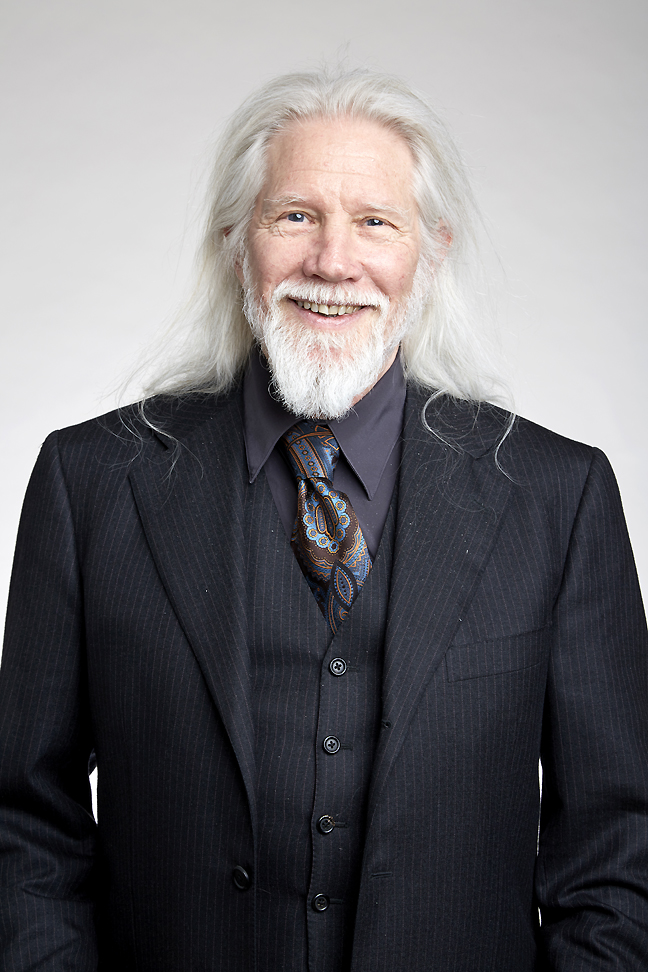
\includegraphics[height=6.0cm, width=4.0cm]{./images/Whitfield_Diffie_Royal_Society.jpg}
        \end{center}
    \end{column}
    \begin{column}{5cm}
        \begin{itemize}
            \item Diffie
        \end{itemize}
    \end{column}
\end{columns}
\end{frame}

\begin{frame}
\frametitle{Presentation}
\framesubtitle{Hellmann}


\end{frame}


\begin{frame}
\frametitle{Presentation}
\framesubtitle{Hellmann}


\end{frame}






\subsection{Tools}



%
% SECTION: Steganography
%
\section{Steganography}
\begin{frame}
    \frametitle{Contents}
    \begin{columns}[t]
        \begin{column}{5cm}
            \tableofcontents[sections={1-3}, currentsection, hideothersubsections]
        \end{column}
        \begin{column}{5cm}
            \tableofcontents[sections={4-5}, currentsection, hideothersubsections]
        \end{column}
    \end{columns}
\end{frame}
\subsection{Related challenge}
\begin{frame}
\frametitle{Related challenges}
\begin{itemize}
    \item \href{https://github.com/cscluxembourg/vestatech/blob/master/challenges/Vesta-asteroid/vesta.png}{Vesta asteroid} - 2 stars.
    \item \href{https://github.com/cscluxembourg/vestatech/blob/master/challenges/sergei/Sergei.png}{Sergei, our chief scientific officer} - 3 stars;
\end{itemize}
\bigskip
How did you solved these challenges?
\end{frame}

\subsection{Presentation}
\begin{frame}[fragile]
\frametitle{Presentation}
\framesubtitle{Steganography}
\begin{itemize}
    \item hiding messages in such a way that no one, apart from the sender and intended recipient, suspects the existence of the message;
    \item a form of security through obscurity;
    \item steganography \textbf{is not} cryptography;
    \item the message can be hidden in different kind of data: pictures, video, sound, network traffic, printed steganography.
    \item different techniques: using metadata, using the red portion of a pixel, Least Significant Bit, etc.
\end{itemize}
\begin{lstlisting}[language=Bash]
$ zip text-to-hide.zip text-to-hide.txt
$ cat song.ogg test-to-hide.zip > song-1.ogg
\end{lstlisting}
\end{frame}



\begin{frame}
\frametitle{A picture can hide a lot of things...}
\framesubtitle{Background picture of the VestaTech challenge platform}
\begin{center}
    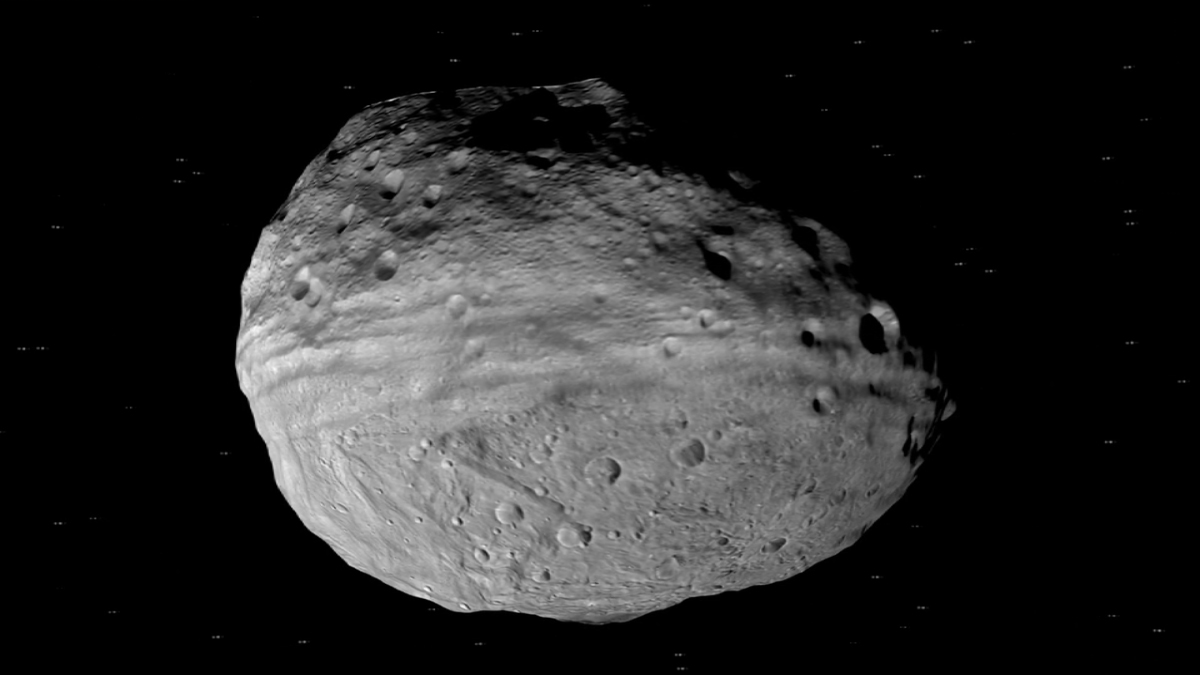
\includegraphics[height=6.2cm, width=12.0cm]{./images/vesta.png}
\end{center}
... thankfully, two gentle clues were placed on the VestaTech website.
\end{frame}

\begin{frame}
\frametitle{Detection - Parity steganalysis}
\begin{center}
    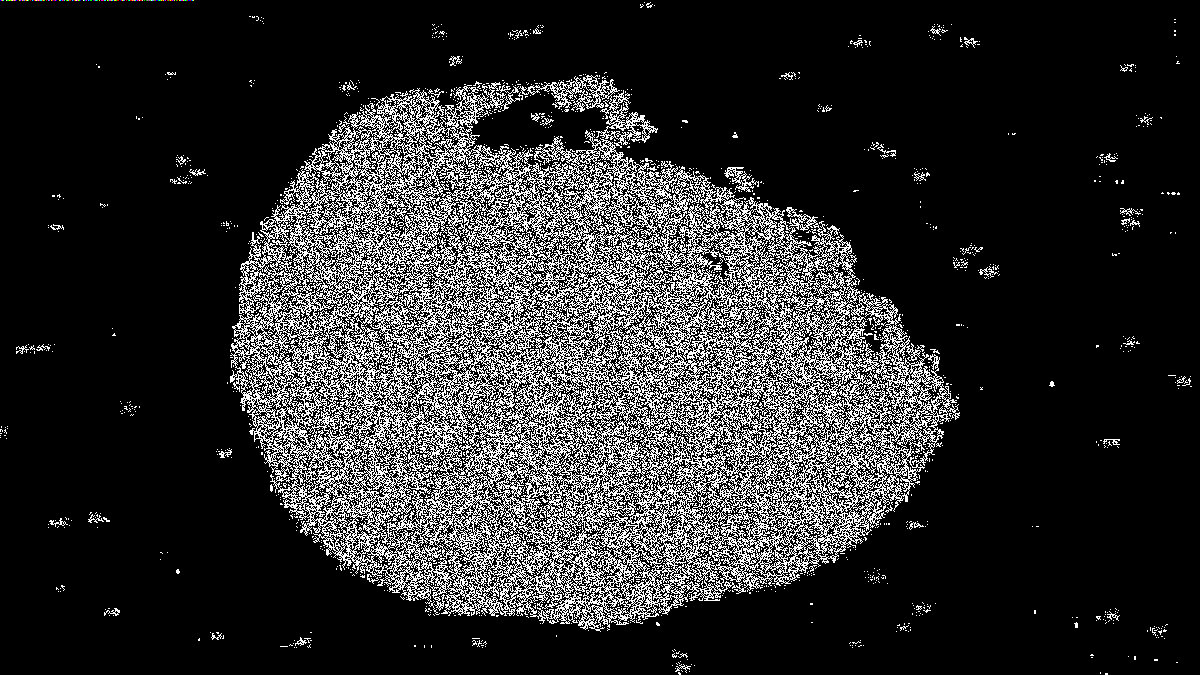
\includegraphics[height=6.0cm, width=12.0cm]{./images/vesta_steg.png}
\end{center}
Replace odd components by 255 and even by 0.

(132, 247, 123) $\longrightarrow$ (0, 255, 255)
\end{frame}

\begin{frame}
\frametitle{Detection - Parity steganalysis}
\begin{center}

\includegraphics[width=12.0cm]{./images/vesta_steg_zoom.png}
\end{center}
\bigskip
So, now?

\bigskip
Try here with this tool: \href{https://stegano-web.herokuapp.com}{https://stegano-web.herokuapp.com}

\bigskip 
Steganalysis is too easy! What can we do? Let put some mess!
\end{frame}

\begin{frame}
\frametitle{Sergei, our chief scientific officer}
\begin{center}
    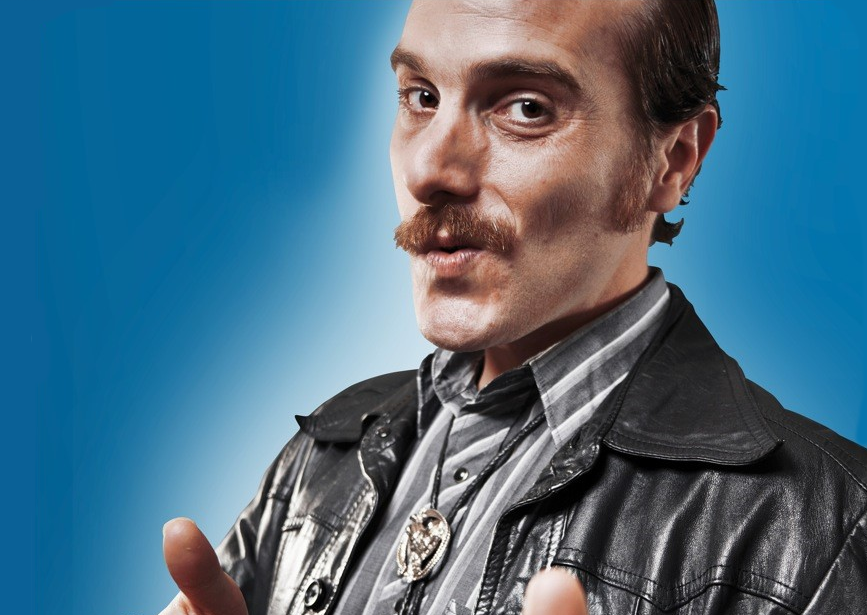
\includegraphics[height=6.0cm, width=10.0cm]{./images/Sergei.png}
\end{center}
\end{frame}

\begin{frame}[fragile]
\frametitle{A pythonic solution}
\begin{lstlisting}[language=Bash]
$ wget https://raw.githubusercontent.com/cscluxembourg/vestatech/master/challenges/sergei/Sergei.png
$ stegano-lsb reveal -i Sergei.png
\end{lstlisting}
Not yet the solution but close... Maybe the metadata will hel you.\\Just saying.
\bigskip

\begin{lstlisting}[language=Bash]
$ stegano-lsb-set reveal -i Sergei.png -g fibonacci -s 9
\end{lstlisting}
\end{frame}

\subsection{Tools}
\begin{frame}
\frametitle{}
\begin{itemize}
    \item \href{https://github.com/topics/steganography}{a lot of tools} are available.
\end{itemize}
\end{frame}



%
% SECTION: Fun with old crypto
%
\section{Fun with old crypto}
\begin{frame}
    \frametitle{Fun with old crypto}
    \begin{columns}[t]
        \begin{column}{5cm}
            \tableofcontents[sections={1-3}, currentsection, hideothersubsections]
        \end{column}
        \begin{column}{5cm}
            \tableofcontents[sections={4-5}, currentsection, hideothersubsections]
        \end{column}
    \end{columns}
\end{frame}
\subsection{Related challenges}
\begin{frame}
\frametitle{Related challenge}
\framesubtitle{Enigma}
\begin{itemize}
    \item \href{https://github.com/cscluxembourg/vestatech/tree/master/challenges/the-missing-piece}{A piece of the prototype is missing} - 1 star;
\end{itemize}
\bigskip
How did you solved this challenge?
\end{frame}

\subsection{Presentation}
\begin{frame}
\frametitle{Presentation}
\framesubtitle{Enigma}
\begin{itemize}
    \item 
\end{itemize}
\end{frame}



\begin{frame}
\frametitle{Solution}
\begin{center}
    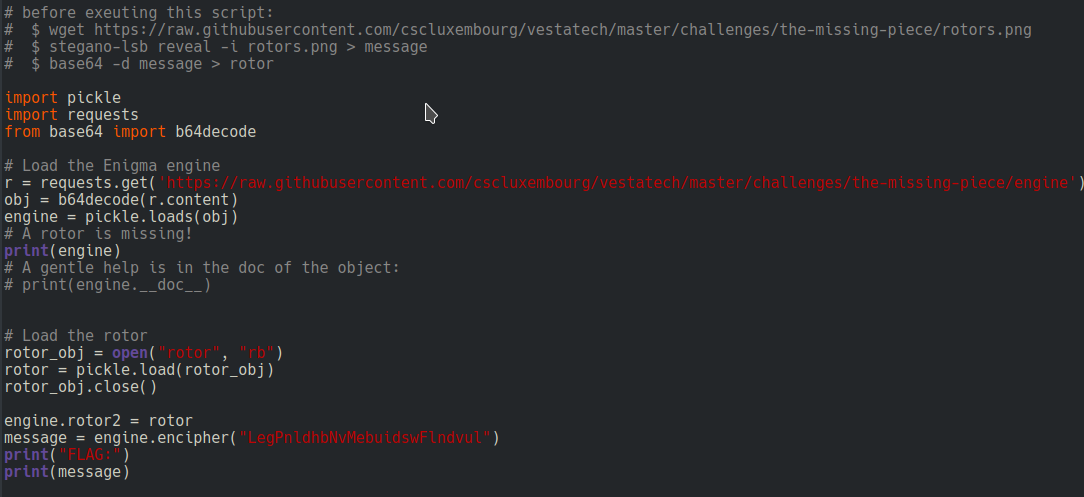
\includegraphics[height=6.5cm, width=12.0cm]{./images/Enigma_solution.png}
\end{center}
\end{frame}



\subsection{Tools}





%
% SECTION: End of the presentation
%
\section*{End of the presentation}
\begin{frame}
    \frametitle{End of the presentation}
    \framesubtitle{Q and A}
    \begin{center}
        \begin{itemize}
            \item Thanks for listening.
            \item Wich challenge did you enjoyed the most?
            \item What's your opinion? Do you want more difficult challenges for the next year?
            \item Any questions?
        \end{itemize}
    \end{center}
\end{frame}
\end{document}
